%%%%%%%%%%%%%%%%%%%%%%%%%%%%%%%%%%%%%%%%%
% Beamer Presentation
% LaTeX Template
% Version 1.0 (10/11/12)
%
% This template has been downloaded from:
% http://www.LaTeXTemplates.com
%
% License:
% CC BY-NC-SA 3.0 (http://creativecommons.org/licenses/by-nc-sa/3.0/)
%
%%%%%%%%%%%%%%%%%%%%%%%%%%%%%%%%%%%%%%%%%

%----------------------------------------------------------------------------------------
%	PACKAGES AND THEMES
%----------------------------------------------------------------------------------------

\documentclass{beamer}

\mode<presentation> {

% The Beamer class comes with a number of default slide themes
% which change the colors and layouts of slides. Below this is a list
% of all the themes, uncomment each in turn to see what they look like.

%\usetheme{default}
%\usetheme{AnnArbor}
%\usetheme{Antibes}
%\usetheme{Bergen}
%\usetheme{Berkeley}
%\usetheme{Berlin}
%\usetheme{Boadilla}
%\usetheme{CambridgeUS}
%\usetheme{Copenhagen}
%\usetheme{Darmstadt}
%\usetheme{Dresden}
%\usetheme{Frankfurt}
%\usetheme{Goettingen}
%\usetheme{Hannover}
%\usetheme{Ilmenau}
%\usetheme{JuanLesPins}
%\usetheme{Luebeck}
\usetheme{Madrid}
%\usetheme{Malmoe}
%\usetheme{Marburg}
%\usetheme{Montpellier}
%\usetheme{PaloAlto}
%\usetheme{Pittsburgh}
%\usetheme{Rochester}
%\usetheme{Singapore}
%\usetheme{Szeged}
%\usetheme{Warsaw}

% As well as themes, the Beamer class has a number of color themes
% for any slide theme. Uncomment each of these in turn to see how it
% changes the colors of your current slide theme.

%\usecolortheme{albatross}
%\usecolortheme{beaver}
%\usecolortheme{beetle}
%\usecolortheme{crane}
%\usecolortheme{dolphin}
%\usecolortheme{dove}
%\usecolortheme{fly}
%\usecolortheme{lily}
%\usecolortheme{orchid}
%\usecolortheme{rose}
%\usecolortheme{seagull}
%\usecolortheme{seahorse}
%\usecolortheme{whale}
%\usecolortheme{wolverine}

%\setbeamertemplate{footline} % To remove the footer line in all slides uncomment this line
%\setbeamertemplate{footline}[page number] % To replace the footer line in all slides with a simple slide count uncomment this line

%\setbeamertemplate{navigation symbols}{} % To remove the navigation symbols from the bottom of all slides uncomment this line
}
\usepackage{verbatim}
\usepackage{fontspec}
\usepackage{tikz}
\setmainfont{DejaVu Sans}
\setmonofont{DejaVu Sans Mono}

\makeatletter
\@ifundefined{lhs2tex.lhs2tex.sty.read}%
  {\@namedef{lhs2tex.lhs2tex.sty.read}{}%
   \newcommand\SkipToFmtEnd{}%
   \newcommand\EndFmtInput{}%
   \long\def\SkipToFmtEnd#1\EndFmtInput{}%
  }\SkipToFmtEnd

\newcommand\ReadOnlyOnce[1]{\@ifundefined{#1}{\@namedef{#1}{}}\SkipToFmtEnd}
\usepackage{amstext}
\usepackage{amssymb}
\usepackage{stmaryrd}
\DeclareFontFamily{OT1}{cmtex}{}
\DeclareFontShape{OT1}{cmtex}{m}{n}
  {<5><6><7><8>cmtex8
   <9>cmtex9
   <10><10.95><12><14.4><17.28><20.74><24.88>cmtex10}{}
\DeclareFontShape{OT1}{cmtex}{m}{it}
  {<-> ssub * cmtt/m/it}{}
\newcommand{\texfamily}{\fontfamily{cmtex}\selectfont}
\DeclareFontShape{OT1}{cmtt}{bx}{n}
  {<5><6><7><8>cmtt8
   <9>cmbtt9
   <10><10.95><12><14.4><17.28><20.74><24.88>cmbtt10}{}
\DeclareFontShape{OT1}{cmtex}{bx}{n}
  {<-> ssub * cmtt/bx/n}{}
\newcommand{\tex}[1]{\text{\texfamily#1}}	% NEU

\newcommand{\Sp}{\hskip.33334em\relax}


\newcommand{\Conid}[1]{\mathit{#1}}
\newcommand{\Varid}[1]{\mathit{#1}}
\newcommand{\anonymous}{\kern0.06em \_}
\newcommand{\plus}{\mathbin{+\!\!\!+}}
\newcommand{\bind}{\mathbin{>\!\!\!>\mkern-6.7mu=}}
\newcommand{\rbind}{\mathbin{=\mkern-6.7mu<\!\!\!<}}% suggested by Neil Mitchell
\newcommand{\sequ}{\mathbin{>\!\!\!>}}
\renewcommand{\leq}{\leqslant}
\renewcommand{\geq}{\geqslant}
\usepackage{polytable}

%mathindent has to be defined
\@ifundefined{mathindent}%
  {\newdimen\mathindent\mathindent\leftmargini}%
  {}%

\def\resethooks{%
  \global\let\SaveRestoreHook\empty
  \global\let\ColumnHook\empty}
\newcommand*{\savecolumns}[1][default]%
  {\g@addto@macro\SaveRestoreHook{\savecolumns[#1]}}
\newcommand*{\restorecolumns}[1][default]%
  {\g@addto@macro\SaveRestoreHook{\restorecolumns[#1]}}
\newcommand*{\aligncolumn}[2]%
  {\g@addto@macro\ColumnHook{\column{#1}{#2}}}

\resethooks

\newcommand{\onelinecommentchars}{\quad-{}- }
\newcommand{\commentbeginchars}{\enskip\{-}
\newcommand{\commentendchars}{-\}\enskip}

\newcommand{\visiblecomments}{%
  \let\onelinecomment=\onelinecommentchars
  \let\commentbegin=\commentbeginchars
  \let\commentend=\commentendchars}

\newcommand{\invisiblecomments}{%
  \let\onelinecomment=\empty
  \let\commentbegin=\empty
  \let\commentend=\empty}

\visiblecomments

\newlength{\blanklineskip}
\setlength{\blanklineskip}{0.66084ex}

\newcommand{\hsindent}[1]{\quad}% default is fixed indentation
\let\hspre\empty
\let\hspost\empty
\newcommand{\NB}{\textbf{NB}}
\newcommand{\Todo}[1]{$\langle$\textbf{To do:}~#1$\rangle$}

\EndFmtInput
\makeatother
%
%
%
%
%
%
% This package provides two environments suitable to take the place
% of hscode, called "plainhscode" and "arrayhscode".
%
% The plain environment surrounds each code block by vertical space,
% and it uses \abovedisplayskip and \belowdisplayskip to get spacing
% similar to formulas. Note that if these dimensions are changed,
% the spacing around displayed math formulas changes as well.
% All code is indented using \leftskip.
%
% Changed 19.08.2004 to reflect changes in colorcode. Should work with
% CodeGroup.sty.
%
\ReadOnlyOnce{polycode.fmt}%
\makeatletter

\newcommand{\hsnewpar}[1]%
  {{\parskip=0pt\parindent=0pt\par\vskip #1\noindent}}

% can be used, for instance, to redefine the code size, by setting the
% command to \small or something alike
\newcommand{\hscodestyle}{}

% The command \sethscode can be used to switch the code formatting
% behaviour by mapping the hscode environment in the subst directive
% to a new LaTeX environment.

\newcommand{\sethscode}[1]%
  {\expandafter\let\expandafter\hscode\csname #1\endcsname
   \expandafter\let\expandafter\endhscode\csname end#1\endcsname}

% "compatibility" mode restores the non-polycode.fmt layout.

\newenvironment{compathscode}%
  {\par\noindent
   \advance\leftskip\mathindent
   \hscodestyle
   \let\\=\@normalcr
   \let\hspre\(\let\hspost\)%
   \pboxed}%
  {\endpboxed\)%
   \par\noindent
   \ignorespacesafterend}

\newcommand{\compaths}{\sethscode{compathscode}}

% "plain" mode is the proposed default.
% It should now work with \centering.
% This required some changes. The old version
% is still available for reference as oldplainhscode.

\newenvironment{plainhscode}%
  {\hsnewpar\abovedisplayskip
   \advance\leftskip\mathindent
   \hscodestyle
   \let\hspre\(\let\hspost\)%
   \pboxed}%
  {\endpboxed%
   \hsnewpar\belowdisplayskip
   \ignorespacesafterend}

\newenvironment{oldplainhscode}%
  {\hsnewpar\abovedisplayskip
   \advance\leftskip\mathindent
   \hscodestyle
   \let\\=\@normalcr
   \(\pboxed}%
  {\endpboxed\)%
   \hsnewpar\belowdisplayskip
   \ignorespacesafterend}

% Here, we make plainhscode the default environment.

\newcommand{\plainhs}{\sethscode{plainhscode}}
\newcommand{\oldplainhs}{\sethscode{oldplainhscode}}
\plainhs

% The arrayhscode is like plain, but makes use of polytable's
% parray environment which disallows page breaks in code blocks.

\newenvironment{arrayhscode}%
  {\hsnewpar\abovedisplayskip
   \advance\leftskip\mathindent
   \hscodestyle
   \let\\=\@normalcr
   \(\parray}%
  {\endparray\)%
   \hsnewpar\belowdisplayskip
   \ignorespacesafterend}

\newcommand{\arrayhs}{\sethscode{arrayhscode}}

% The mathhscode environment also makes use of polytable's parray
% environment. It is supposed to be used only inside math mode
% (I used it to typeset the type rules in my thesis).

\newenvironment{mathhscode}%
  {\parray}{\endparray}

\newcommand{\mathhs}{\sethscode{mathhscode}}

% texths is similar to mathhs, but works in text mode.

\newenvironment{texthscode}%
  {\(\parray}{\endparray\)}

\newcommand{\texths}{\sethscode{texthscode}}

% The framed environment places code in a framed box.

\def\codeframewidth{\arrayrulewidth}
\RequirePackage{calc}

\newenvironment{framedhscode}%
  {\parskip=\abovedisplayskip\par\noindent
   \hscodestyle
   \arrayrulewidth=\codeframewidth
   \tabular{@{}|p{\linewidth-2\arraycolsep-2\arrayrulewidth-2pt}|@{}}%
   \hline\framedhslinecorrect\\{-1.5ex}%
   \let\endoflinesave=\\
   \let\\=\@normalcr
   \(\pboxed}%
  {\endpboxed\)%
   \framedhslinecorrect\endoflinesave{.5ex}\hline
   \endtabular
   \parskip=\belowdisplayskip\par\noindent
   \ignorespacesafterend}

\newcommand{\framedhslinecorrect}[2]%
  {#1[#2]}

\newcommand{\framedhs}{\sethscode{framedhscode}}

% The inlinehscode environment is an experimental environment
% that can be used to typeset displayed code inline.

\newenvironment{inlinehscode}%
  {\(\def\column##1##2{}%
   \let\>\undefined\let\<\undefined\let\\\undefined
   \newcommand\>[1][]{}\newcommand\<[1][]{}\newcommand\\[1][]{}%
   \def\fromto##1##2##3{##3}%
   \def\nextline{}}{\) }%

\newcommand{\inlinehs}{\sethscode{inlinehscode}}

% The joincode environment is a separate environment that
% can be used to surround and thereby connect multiple code
% blocks.

\newenvironment{joincode}%
  {\let\orighscode=\hscode
   \let\origendhscode=\endhscode
   \def\endhscode{\def\hscode{\endgroup\def\@currenvir{hscode}\\}\begingroup}
   %\let\SaveRestoreHook=\empty
   %\let\ColumnHook=\empty
   %\let\resethooks=\empty
   \orighscode\def\hscode{\endgroup\def\@currenvir{hscode}}}%
  {\origendhscode
   \global\let\hscode=\orighscode
   \global\let\endhscode=\origendhscode}%

\makeatother
\EndFmtInput
%



\usepackage{graphicx} % Allows including images
\usepackage{booktabs} % Allows the use of \toprule, \midrule and \bottomrule in tables


\usetikzlibrary{arrows}

\tikzset{
  treenode/.style = {align=center, inner sep=0pt, text centered,
    font=\sffamily},
  arn_n/.style = {treenode, circle, black font=\sffamily\bfseries, draw=black,
    fill=white, text width=1.5em},% arbre rouge noir, noeud noir
  arn_r/.style = {treenode, circle, red, draw=red, 
    text width=1.5em, very thick},% arbre rouge noir, noeud rouge
  arn_x/.style = {treenode, rectangle, draw=black,
    minimum width=0.5em, minimum height=0.5em}% arbre rouge noir, nil
}


\usepackage{tkz-graph}

\tikzset{
  LabelStyle/.style = { rectangle, rounded corners, draw,
                        minimum width = 2em, fill = yellow!50,
                        text = red, font = \bfseries },
  VertexStyle/.append style = { inner sep=5pt,
                                font = \Large\bfseries},
  EdgeStyle/.append style = {->, bend left} 
}

%----------------------------------------------------------------------------------------
%	TITLE PAGE
%----------------------------------------------------------------------------------------

\title[Verified Structures in Agda - Progress]{Verified Data Structures and Algorithms in Agda  Progress Report} % The short title appears at the bottom of every slide, the full title is only on the title page

\author{Razvan Kusztos\\Supervisor: Dr. Timothy Griffin} % Your name
\institute[rek43] % Your institution as it will appear on the bottom of every slide, may be shorthand to save space
{
University of Cambridge \\ % Your institution for the title page
\medskip
\textit{Part II} % Your email address
}
\date{\today} % Date, can be changed to a custom date

\begin{document}


%----------------------------------------------------------------------------------------
%	PRESENTATION SLIDES
%----------------------------------------------------------------------------------------


\begin{frame}
\titlepage % Print the title page as the first slide
\end{frame}


\begin{frame}
\frametitle{Motivation} 
\begin{itemize} 
\item Dependent typing enforces correctness of programs.
\item Nested types maintain invariants of data structure.
\item Together they present a challenge both for programming and verifying correctness
\item The dissertation's purpose was: 
\item \hspace{5mm} Implementing the Finger Tree in agda
\item \hspace{5mm} 	Proving the correctness of its methods. 
\end{itemize} 

\end{frame}


%\begin{frame}
%\frametitle{Dependent Typing} 
%
%\begin{itemize}
%\item{Types can depend of values} 
%\item{Can help us enforce invariants of our data structures}
%\item{Rules out a number of programming errors at compile time}  
%\item{Example: list versus vector}  
%\end{itemize} 
%
%\begin{hscode}\SaveRestoreHook
%\column{B}{@{}>{\hspre}l<{\hspost}@{}}%
%\column{5}{@{}>{\hspre}l<{\hspost}@{}}%
%\column{7}{@{}>{\hspre}l<{\hspost}@{}}%
%\column{E}{@{}>{\hspre}l<{\hspost}@{}}%
%\>[5]{}\mathbf{data}\;\Conid{List}\;(\Conid{A}\mathbin{:}\Conid{Set})\mathbin{:}\Conid{Set}\;\mathbf{where}{}\<[E]%
%\\
%\>[5]{}\hsindent{2}{}\<[7]%
%\>[7]{}[\mskip1.5mu \mskip1.5mu]\mathbin{:}\Conid{List}\;\Conid{A}{}\<[E]%
%\\
%\>[5]{}\hsindent{2}{}\<[7]%
%\>[7]{}\anonymous \mathbin{∷\char95 }\mathbin{:}\Conid{A}\mathbin{→}\Conid{List}\;\Conid{A}\mathbin{→}\Conid{List}\;\Conid{A}{}\<[E]%
%\ColumnHook
%\end{hscode}\resethooks
%
%\begin{hscode}\SaveRestoreHook
%\column{B}{@{}>{\hspre}l<{\hspost}@{}}%
%\column{5}{@{}>{\hspre}l<{\hspost}@{}}%
%\column{7}{@{}>{\hspre}l<{\hspost}@{}}%
%\column{E}{@{}>{\hspre}l<{\hspost}@{}}%
%\>[5]{}\mathbf{data}\;\Conid{Vec}\;(\Conid{A}\mathbin{:}\Conid{Set})\mathbin{:}\Conid{ℕ}\mathbin{→}\Conid{Set}\;\mathbf{where}{}\<[E]%
%\\
%\>[5]{}\hsindent{2}{}\<[7]%
%\>[7]{}[\mskip1.5mu \mskip1.5mu]\mathbin{:}\Conid{Vec}\;\Conid{A}\;\mathrm{0}{}\<[E]%
%\\
%\>[5]{}\hsindent{2}{}\<[7]%
%\>[7]{}\anonymous \mathbin{∷\char95 }\mathbin{:}\mathbin{∀}\{\mskip1.5mu \Varid{n}\mskip1.5mu\}\mathbin{→}\Conid{A}\mathbin{→}\Conid{Vec}\;\Conid{A}\;\Varid{n}\mathbin{→}\Conid{Vec}\;\Conid{A}\;(\Varid{suc}\;\Varid{n}){}\<[E]%
%\\
%\>[5]{}\Varid{open}\;\mathbf{import}\;\Conid{\Conid{Data}.Product}{}\<[E]%
%\ColumnHook
%\end{hscode}\resethooks
%
%\end{frame} 
%
%\begin{frame}
%\frametitle{Propositions as Types} 
%
%\begin{itemize}
%\item Increase the expresiveness of programs
%\item In particular, under the Curry Howard Isomorphism, programs become proofs.
%\item Example: Equality relation between types: 
%\end{itemize} 
%
%\begin{hscode}\SaveRestoreHook
%\column{B}{@{}>{\hspre}l<{\hspost}@{}}%
%\column{3}{@{}>{\hspre}l<{\hspost}@{}}%
%\column{E}{@{}>{\hspre}l<{\hspost}@{}}%
%\>[B]{}\Varid{open}\;\mathbf{import}\;\Conid{Level}{}\<[E]%
%\\
%\>[B]{}\mathbf{data}\;\anonymous \mathbin{≡\char95}\{\mskip1.5mu \Varid{a}\mathbin{:}\Conid{Level}\mskip1.5mu\}\;\{\mskip1.5mu \Conid{A}\mathbin{:}\Conid{Set}\;\Varid{a}\mskip1.5mu\}\;(\Varid{x}\mathbin{:}\Conid{A})\mathbin{:}\Conid{A}\mathbin{→}\Conid{Set}\;\Varid{a}\;\mathbf{where}{}\<[E]%
%\\
%\>[B]{}\hsindent{3}{}\<[3]%
%\>[3]{}\Varid{refl}\mathbin{:}\Varid{x}\mathbin{≡}\Varid{x}{}\<[E]%
%\ColumnHook
%\end{hscode}\resethooks
%\end{frame} 
%
%
%\begin{frame}
%\frametitle{Example proof by induction} 
% 
%\begin{hscode}\SaveRestoreHook
%\column{B}{@{}>{\hspre}l<{\hspost}@{}}%
%\column{3}{@{}>{\hspre}l<{\hspost}@{}}%
%\column{E}{@{}>{\hspre}l<{\hspost}@{}}%
%\>[3]{}\Varid{open}\;\mathbf{import}\;\Conid{\Conid{Relation}.\Conid{Binary}.PropositionalEquality}{}\<[E]%
%\\[\blanklineskip]%
%\>[3]{}\mathbin{+}\Varid{assoc}\mathbin{:}\mathbin{∀}(\Varid{x}\;\Varid{y}\;\Varid{z}\mathbin{:}\Conid{ℕ})\mathbin{→}(\Varid{x}\mathbin{+}(\Varid{y}\mathbin{+}\Varid{z}))\mathbin{≡}((\Varid{x}\mathbin{+}\Varid{y})\mathbin{+}\Varid{z}){}\<[E]%
%\\
%\>[3]{}\mathbin{+}\Varid{assoc}\;\Varid{zero}\;\Varid{y}\;\Varid{z}\mathrel{=}\Varid{refl}{}\<[E]%
%\\
%\>[3]{}\mathbin{+}\Varid{assoc}\;(\Varid{suc}\;\Varid{x})\;\Varid{y}\;\Varid{z}\;\Varid{rewrite}\mathbin{+}\Varid{assoc}\;\Varid{x}\;\Varid{y}\;\Varid{z}\mathrel{=}\Varid{refl}{}\<[E]%
%\ColumnHook
%\end{hscode}\resethooks 
%
%\end{frame} 

\begin{frame} 
\frametitle{Regular vs Nested Types} 


\textit{List} is an example of a \textbf{regular} data type. \\~\\
One can also declare \textbf{irregular (nested)} data types \cite{nested}, where the recursive call to the type constructor takes as argument a different type (examples to follow)\\~\\

In older versions of Haskell and ML, although the declarations are valid, one couldn't write functions to operate on them. \cite{nested} (Hindley-Milner typing).\\~\\
They turn out to be very useful in practice, as they can keep strong invariants on the data. \\ 
\end{frame} 

\begin{frame} 
\frametitle{Example 1: Full binary tree} 
	\begin{hscode}\SaveRestoreHook
	\column{B}{@{}>{\hspre}l<{\hspost}@{}}%
	\column{3}{@{}>{\hspre}l<{\hspost}@{}}%
	\column{5}{@{}>{\hspre}l<{\hspost}@{}}%
	\column{E}{@{}>{\hspre}l<{\hspost}@{}}%
	\>[3]{}\mathbf{data}\;\Conid{Nest}\;(\Conid{A}\mathbin{:}\Conid{Set})\mathbin{:}\Conid{Set}\;\mathbf{where}{}\<[E]%
	\\
	\>[3]{}\hsindent{2}{}\<[5]%
	\>[5]{}\Conid{Nil}\mathbin{:}\Conid{Nest}\;\Conid{A}{}\<[E]%
	\\
	\>[3]{}\hsindent{2}{}\<[5]%
	\>[5]{}\Conid{Cons}\mathbin{:}\Conid{A}\mathbin{→}\Conid{Nest}\;(\Conid{A}\mathbin{×}\Conid{A})\mathbin{→}\Conid{Nest}\;\Conid{A}{}\<[E]%
	\ColumnHook
	\end{hscode}\resethooks

	\begin{hscode}\SaveRestoreHook
	\column{B}{@{}>{\hspre}l<{\hspost}@{}}%
	\column{3}{@{}>{\hspre}l<{\hspost}@{}}%
	\column{E}{@{}>{\hspre}l<{\hspost}@{}}%
	\>[3]{}\Varid{ex}\mathbin{:}\Conid{Nest}\;\Conid{ℕ}{}\<[E]%
	\\
	\>[3]{}\Varid{ex}\mathrel{=}\Conid{Cons}\;\mathrm{1}\;(\Conid{Cons}\;(\mathrm{2},\mathrm{3})\;(\Conid{Cons}\;((\mathrm{4},\mathrm{5}),(\mathrm{6},\mathrm{7}))\;\Conid{Nil})){}\<[E]%
	\ColumnHook
	\end{hscode}\resethooks

	\begin{center}
	
		\begin{tikzpicture} [scale = 0.7,level 1/.style = {sibling distance = 5cm, level distance = 1.5cm},
							  level 2/.style = {sibling distance = 3cm}]
		\node [arn_n] {1}
		 child{ node [arn_n] {2} 
		            child{node [arn_n] {4}} 
		            child{node [arn_n] {5}}	
		      }
		 child{node [arn_n] {3} 
		            child{node [arn_n] {6}} 
		            child{node [arn_n] {7}}	
		      };
		\end{tikzpicture}
	
	\end{center} 



\end{frame} 


\begin{frame}
\frametitle{Example 2: Cyclic list \cite{cyclic}} 
\begin{hscode}\SaveRestoreHook
\column{B}{@{}>{\hspre}l<{\hspost}@{}}%
\column{3}{@{}>{\hspre}l<{\hspost}@{}}%
\column{6}{@{}>{\hspre}l<{\hspost}@{}}%
\column{E}{@{}>{\hspre}l<{\hspost}@{}}%
\>[3]{}\mathbf{data}\;\Conid{Clist}\;(\Conid{A}\mathbin{:}\Conid{Set})\mathbin{:}\Conid{Set}\;\mathbf{where}{}\<[E]%
\\
\>[3]{}\hsindent{3}{}\<[6]%
\>[6]{}\Conid{Var}\mathbin{:}\Conid{A}\mathbin{→}\Conid{Clist}\;\Conid{A}{}\<[E]%
\\
\>[3]{}\hsindent{3}{}\<[6]%
\>[6]{}\Conid{Nil}\mathbin{:}\Conid{Clist}\;\Conid{A}{}\<[E]%
\\
\>[3]{}\hsindent{3}{}\<[6]%
\>[6]{}\Conid{RCons}\mathbin{:}\Conid{ℕ}\mathbin{→}\Conid{Clist}\;(\Conid{Maybe}\;\Conid{A})\mathbin{→}\Conid{Clist}\;\Conid{A}{}\<[E]%
\ColumnHook
\end{hscode}\resethooks

\begin{hscode}\SaveRestoreHook
\column{B}{@{}>{\hspre}l<{\hspost}@{}}%
\column{4}{@{}>{\hspre}l<{\hspost}@{}}%
\column{E}{@{}>{\hspre}l<{\hspost}@{}}%
\>[4]{}\Varid{ex}\mathbin{:}\Conid{CList}\;(){}\<[E]%
\\
\>[4]{}\Varid{clist2}\mathrel{=}\Conid{RCons}\;\mathrm{1}\;(\Conid{RCons2}\;(\Conid{RCons}\;\mathrm{3}\;(\Conid{Var}\;(\Varid{just}\;\Varid{nothing})))){}\<[E]%
\ColumnHook
\end{hscode}\resethooks

\begin{center} 

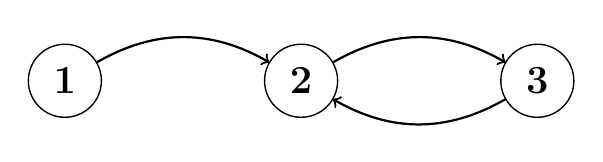
\begin{tikzpicture}
  \SetGraphUnit{3}
  \Vertex{2}
  \WE(2){1}
  \EA(2){3}
  \Edge(1)(2)
  \Edge(2)(3)
  \Edge(3)(2)
%  \Edge(A)(B)
\end{tikzpicture}

\end{center} 
\end{frame} 

\begin{frame} 
\frametitle{Example 3: Finger Trees}

% full declaration  
%\begin{hscode}\SaveRestoreHook
%\column{B}{@{}>{\hspre}l<{\hspost}@{}}%
%\column{3}{@{}>{\hspre}l<{\hspost}@{}}%
%\column{5}{@{}>{\hspre}l<{\hspost}@{}}%
%\column{7}{@{}>{\hspre}l<{\hspost}@{}}%
%\column{13}{@{}>{\hspre}l<{\hspost}@{}}%
%\column{14}{@{}>{\hspre}l<{\hspost}@{}}%
%\column{16}{@{}>{\hspre}l<{\hspost}@{}}%
%\column{E}{@{}>{\hspre}l<{\hspost}@{}}%
%\>[3]{}\mathbf{module}\;\Varid{fingertree}\;\mathbf{where}{}\<[E]%
%\\[\blanklineskip]%
%\>[3]{}\hsindent{2}{}\<[5]%
%\>[5]{}\mathbf{data}\;\Conid{Node}\;\{\mskip1.5mu \Varid{a}\mskip1.5mu\}\;(\Conid{A}\mathbin{:}\Conid{Set}\;\Varid{a})\mathbin{:}\Conid{Set}\;\Varid{a}\;\mathbf{where}{}\<[E]%
%\\
%\>[5]{}\hsindent{2}{}\<[7]%
%\>[7]{}\Conid{Node2}\mathbin{:}\Conid{A}\mathbin{→}\Conid{A}\mathbin{→}\Conid{Node}\;\Conid{A}{}\<[E]%
%\\
%\>[5]{}\hsindent{2}{}\<[7]%
%\>[7]{}\Conid{Node3}\mathbin{:}\Conid{A}\mathbin{→}\Conid{A}\mathbin{→}\Conid{A}\mathbin{→}\Conid{Node}\;\Conid{A}{}\<[E]%
%\\[\blanklineskip]%
%\>[3]{}\hsindent{2}{}\<[5]%
%\>[5]{}\mathbf{data}\;\Conid{Digit}\;\{\mskip1.5mu \Varid{a}\mskip1.5mu\}\;(\Conid{A}\mathbin{:}\Conid{Set}\;\Varid{a})\mathbin{:}\Conid{Set}\;\Varid{a}\;\mathbf{where}{}\<[E]%
%\\
%\>[5]{}\hsindent{2}{}\<[7]%
%\>[7]{}\Conid{One}{}\<[13]%
%\>[13]{}\mathbin{:}\Conid{A}\mathbin{→}\Conid{Digit}\;\Conid{A}{}\<[E]%
%\\
%\>[5]{}\hsindent{2}{}\<[7]%
%\>[7]{}\Conid{Two}{}\<[13]%
%\>[13]{}\mathbin{:}\Conid{A}\mathbin{→}\Conid{A}\mathbin{→}\Conid{Digit}\;\Conid{A}{}\<[E]%
%\\
%\>[5]{}\hsindent{2}{}\<[7]%
%\>[7]{}\Conid{Three}\mathbin{:}\Conid{A}\mathbin{→}\Conid{A}\mathbin{→}\Conid{A}\mathbin{→}\Conid{Digit}\;\Conid{A}{}\<[E]%
%\\
%\>[5]{}\hsindent{2}{}\<[7]%
%\>[7]{}\Conid{Four}{}\<[13]%
%\>[13]{}\mathbin{:}\Conid{A}\mathbin{→}\Conid{A}\mathbin{→}\Conid{A}\mathbin{→}\Conid{A}\mathbin{→}\Conid{Digit}\;\Conid{A}{}\<[E]%
%\\[\blanklineskip]%
%\>[3]{}\hsindent{2}{}\<[5]%
%\>[5]{}\mathbf{data}\;\Conid{FingerTree}\;\{\mskip1.5mu \Varid{a}\mskip1.5mu\}\;(\Conid{A}\mathbin{:}\Conid{Set}\;\Varid{a})\mathbin{:}\Conid{Set}\;\Varid{a}\;\mathbf{where}{}\<[E]%
%\\
%\>[5]{}\hsindent{2}{}\<[7]%
%\>[7]{}\Conid{Empty}{}\<[14]%
%\>[14]{}\mathbin{:}\Conid{FingerTree}\;\Conid{A}{}\<[E]%
%\\
%\>[5]{}\hsindent{2}{}\<[7]%
%\>[7]{}\Conid{Single}\mathbin{:}\Conid{A}\mathbin{→}\Conid{FingerTree}\;\Conid{A}{}\<[E]%
%\\
%\>[5]{}\hsindent{2}{}\<[7]%
%\>[7]{}\Conid{Deep}{}\<[14]%
%\>[14]{}\mathbin{:}\Conid{Digit}\;\Conid{A}\mathbin{→}\Conid{FingerTree}\;(\Conid{Node}\;\Conid{A})\mathbin{→}\Conid{Digit}\;\Conid{A}\mathbin{→}{}\<[E]%
%\\
%\>[14]{}\hsindent{2}{}\<[16]%
%\>[16]{}\Conid{FingerTree}\;\Conid{A}{}\<[E]%
%\ColumnHook
%\end{hscode}\resethooks

%just the fingertree
  \begin{hscode}\SaveRestoreHook
\column{B}{@{}>{\hspre}l<{\hspost}@{}}%
\column{5}{@{}>{\hspre}l<{\hspost}@{}}%
\column{7}{@{}>{\hspre}l<{\hspost}@{}}%
\column{14}{@{}>{\hspre}l<{\hspost}@{}}%
\column{16}{@{}>{\hspre}l<{\hspost}@{}}%
\column{E}{@{}>{\hspre}l<{\hspost}@{}}%
\>[5]{}\mathbf{data}\;\Conid{FingerTree}\;\{\mskip1.5mu \Varid{a}\mskip1.5mu\}\;(\Conid{A}\mathbin{:}\Conid{Set}\;\Varid{a})\mathbin{:}\Conid{Set}\;\Varid{a}\;\mathbf{where}{}\<[E]%
\\
\>[5]{}\hsindent{2}{}\<[7]%
\>[7]{}\Conid{Empty}{}\<[14]%
\>[14]{}\mathbin{:}\Conid{FingerTree}\;\Conid{A}{}\<[E]%
\\
\>[5]{}\hsindent{2}{}\<[7]%
\>[7]{}\Conid{Single}\mathbin{:}\Conid{A}\mathbin{→}\Conid{FingerTree}\;\Conid{A}{}\<[E]%
\\
\>[5]{}\hsindent{2}{}\<[7]%
\>[7]{}\Conid{Deep}{}\<[14]%
\>[14]{}\mathbin{:}\Conid{Digit}\;\Conid{A}\mathbin{→}\Conid{FingerTree}\;(\Conid{Node}\;\Conid{A})\mathbin{→}\Conid{Digit}\;\Conid{A}\mathbin{→}{}\<[E]%
\\
\>[14]{}\hsindent{2}{}\<[16]%
\>[16]{}\Conid{FingerTree}\;\Conid{A}{}\<[E]%
\ColumnHook
\end{hscode}\resethooks

\end{frame} 


\begin{frame}
\frametitle{Motivation} 
The original paper suggests implementing Views \cite{wadler} in order to make implementations more straight-forward, while keeping the same complexity. \\~\\
 \begin{hscode}\SaveRestoreHook
\column{B}{@{}>{\hspre}l<{\hspost}@{}}%
\column{5}{@{}>{\hspre}l<{\hspost}@{}}%
\column{7}{@{}>{\hspre}l<{\hspost}@{}}%
\column{E}{@{}>{\hspre}l<{\hspost}@{}}%
\>[5]{}\mathbf{data}\;\Conid{ViewL}\;\{\mskip1.5mu \Varid{a}\mskip1.5mu\}\;(\Conid{A}\mathbin{:}\Conid{Set}\;\Varid{a})\mathbin{:}\Conid{Set}\;\Varid{a}\;\mathbf{where}{}\<[E]%
\\
\>[5]{}\hsindent{2}{}\<[7]%
\>[7]{}\Varid{nilL}\mathbin{:}\Conid{ViewL}\;\Conid{A}{}\<[E]%
\\
\>[5]{}\hsindent{2}{}\<[7]%
\>[7]{}\Varid{consL}\mathbin{:}\Conid{A}\mathbin{→}\Conid{FingerTree}\;\Conid{A}\mathbin{→}\Conid{ViewL}\;\Conid{A}{}\<[E]%
\ColumnHook
\end{hscode}\resethooks

And a function to transform between the views.

  \begin{hscode}\SaveRestoreHook
\column{B}{@{}>{\hspre}l<{\hspost}@{}}%
\column{5}{@{}>{\hspre}l<{\hspost}@{}}%
\column{21}{@{}>{\hspre}c<{\hspost}@{}}%
\column{21E}{@{}l@{}}%
\column{E}{@{}>{\hspre}l<{\hspost}@{}}%
\>[5]{}\Varid{viewL}\mathbin{:}\mathbin{∀}\{\mskip1.5mu \Varid{a}\mskip1.5mu\}\;\{\mskip1.5mu \Conid{A}\mathbin{:}\Conid{Set}\;\Varid{a}\mskip1.5mu\}\mathbin{→}\Conid{FingerTree}\;\Conid{A}\mathbin{→}\Conid{ViewL}\;\Conid{A}{}\<[E]%
\\
\>[5]{}\Varid{viewL}\;\Varid{ft}\mathrel{=}\{\mskip1.5mu \mathbin{!}{}\<[21]%
\>[21]{}\mathbin{!}\mskip1.5mu\}{}\<[21E]%
\ColumnHook
\end{hscode}\resethooks


\end{frame}

 
\begin{frame} 
\frametitle{Motivation}
However, implementing functions stops working because of termination checker.

  \begin{hscode}\SaveRestoreHook
\column{B}{@{}>{\hspre}l<{\hspost}@{}}%
\column{5}{@{}>{\hspre}l<{\hspost}@{}}%
\column{E}{@{}>{\hspre}l<{\hspost}@{}}%
\>[5]{}\Varid{reverse}\mathbin{:}\mathbin{∀}\{\mskip1.5mu \Varid{a}\mskip1.5mu\}\;\{\mskip1.5mu \Conid{A}\mathbin{:}\Conid{Set}\;\Varid{a}\mskip1.5mu\}\mathbin{→}\Conid{FingerTree}\;\Conid{A}\mathbin{→}\Conid{FingerTree}\;\Conid{A}{}\<[E]%
\\
\>[5]{}\Varid{reverse}\;\Varid{ft}\;\Varid{with}\;\Varid{viewL}\;\Varid{ft}{}\<[E]%
\\
\>[5]{}\Varid{reverse}\;\Varid{ft}\mid \Varid{nilL}\mathrel{=}\Varid{ft}{}\<[E]%
\\
\>[5]{}\Varid{reverse}\;\Varid{ft}\mid \Varid{consL}\;\Varid{x}\;\Varid{xs}\mathrel{=}(\Varid{reverse}\;\Varid{xs})\mathbin{▷}\Varid{x}{}\<[E]%
\ColumnHook
\end{hscode}\resethooks
\end{frame} 

%\begin{frame} 
%\frametitle{Termination} 
%In order for Agda to be consistent, it needs to not allow programs to loop forever.
%Termination is undecidable, therefore heuristics are employed.
%Agda's heuristic is based on 'structurally smaller arguments' in each recursive call.
%There is a number of ways of convincing agda that arguments get structurally smaller: 
%\begin{itemize}
%\item Using Sized types, the builtin system.
%\item The same principle: index data structure with an arbitrary type that gets structurally smaller.
%\item Defining a well-founded relation between arguments, and using the principles of WF-induction.
%\end{itemize} 


\begin{frame} 
\frametitle{Progress Made - Implementation} 

\begin{itemize}
\item Implemented the FingerTree in 3 iterations with operations like reduce, view, append etc.
\item \hspace{5mm} 1. The plain, non-dependent one (the declaration of which was above)
\item \hspace{5mm} 2. A modification that includes the concept of a measurement \cite{rpat} 
\item \hspace{5mm} 3. A dependent version of the second one.
\end{itemize} 

\end{frame} 

\begin{frame}
\frametitle{Progress Made - Verification} 
\begin{itemize} 
\vspace{5mm}
\item The dependent implementation contains internal verification of the axioms measurement should entail
\vspace{5mm}
\item Wrote proofs of correctness for the cons operator.
\vspace{5mm} 
\item Specialized the data structure through measurements (e.g. Random Access Sequence). 
\vspace{5mm}
\item Implemented a 4th version of the FingerTree, following an Isabelle implementation \cite{isabelle}, that has a very different approach
\end{itemize}
\end{frame}

\begin{frame}
\frametitle{Progress Made - Overcoming Difficulties} 
\begin{itemize}
\item Using the principle of WF induction, I could write an implementation of the reverse function.
\vspace{5mm}
\item I have presented an argument that Sized types cannot be used in this context.
\end{itemize} 
\end{frame}

\begin{frame}
\frametitle{Further work} 
\begin{itemize}
\item Produce more correctness proofs: 
\item Evaluate by seeing whether the dependent version hinders amortized performance (which is amortized O(1) for most operations \cite{okasaki})
\item Explore the performance difference between the original and the isabelle implementation. 
\item Provide a more convincing argument that Sizes cannot be employed here.
\item Attempt to generalize for other nested data structures \cite{numerical}. 
\end{itemize} 
\end{frame} 


\begin{frame}
\frametitle{References}
\footnotesize{
\begin{thebibliography}{99} % Beamer does not support BibTeX so references must be inserted manually as below
\bibitem[0]{nested} Richard Bird and Lambert Meertens
\newblock Nested Datatypes 

\bibitem[1]{numerical} Ralf Hinze
\newblock Numerical Representations as Higher Order Nested Datatypes.

\bibitem[2]{okasaki} Chris Okasaki (1996)
\newblock Purely Functional Data Structures 
\bibitem[3]{rpat} Ralf Hinze and Ross Paterson (2006)
\newblock Finger Trees: A Simple General-purpose Data Structure
\newblock \emph{Journal of Functional Programming } 16(2):197–217.

\bibitem[4]{isabelle} Benedikt Nordho, Stefan Korner, Peter Lammich (2014)
\newblock FingerTrees 

\bibitem[5]{cyclic} Neil Ghani, Makoto Hamana, Tarmo Uustalu, Varmo Vene (2006)
\newblock Representing Cyclic Structures as Nested Datatypes  

\bibitem[6]{wadler} Phil Wadler (1986)
\newblock Views: A way for pattern matching to cohabit with data abstraction 





\end{thebibliography}
}
\end{frame}

%------------------------------------------------

\begin{frame}
\Huge{\centerline{Thank you!}}
\end{frame}

%----------------------------------------------------------------------------------------

\end{document}
